\documentclass{article}
% fonts
\usepackage[scaled=0.92]{helvet}   % set Helvetica as the sans-serif font
\renewcommand{\rmdefault}{ptm}     % set Times as the default text font

% dmb: not mandatory, but i recommend you use mtpro for math fonts.
% there is a free version called mtprolite.

% \usepackage[amssymbols,subscriptcorrection,slantedGreek,nofontinfo]{mtpro2}

\usepackage[T1]{fontenc}
\usepackage{amsmath}
\usepackage{amsfonts}
\usepackage{tikz}


% page numbers
\usepackage{fancyhdr}
\fancypagestyle{newstyle}{
\fancyhf{} % clear all header and footer fields
\fancyfoot[R]{\vspace{0.1in} \small \thepage}
\renewcommand{\headrulewidth}{0pt}
\renewcommand{\footrulewidth}{0pt}}
\pagestyle{newstyle}

% geometry of the page
\usepackage[top=1in, bottom=1in, left=1.625in, right=1.625in]{geometry}

% for enumerate* and itemize*
\usepackage{mdwlist}

% paragraph spacing
\setlength{\parindent}{0pt}
\setlength{\parskip}{2ex plus 0.4ex minus 0.2ex}

% useful packages
\usepackage{natbib}
\usepackage{epsfig}
\usepackage{url}
\usepackage{bm}

\usetikzlibrary{fit}
\usetikzlibrary{calc}
\usepackage{graphicx}

\usepackage{algorithmic}
\usepackage{amstext}
\usepackage{tikz}
\usetikzlibrary{arrows,decorations.pathmorphing,fit,positioning}

\newcommand{\dir}{\text{Dirichlet}}
\newcommand{\mult}{\text{Multinomial}}


\begin{document}

\begin{center}
	\textbf{Gibbs Sampler} \\
	Prateek Gupta \\
	\today
\end{center}

\textbf{Reading response}

I got a burning phase of 1000 iterations after which change in log likelihood was of only 2.00 while the total log likelihood was around -400.0. Not going beyond the computing capacity I took number of clusters as 10 and sampled total of 100 points. The end result indicates that it can recognize only fewer number of clusters. It seems like when there is not much data from each clusters it groups those clusters. This can be interpreted as hierarchy on groups.  My guess is that more number of points per cluster will result in better clustering.  

\begin{figure}
	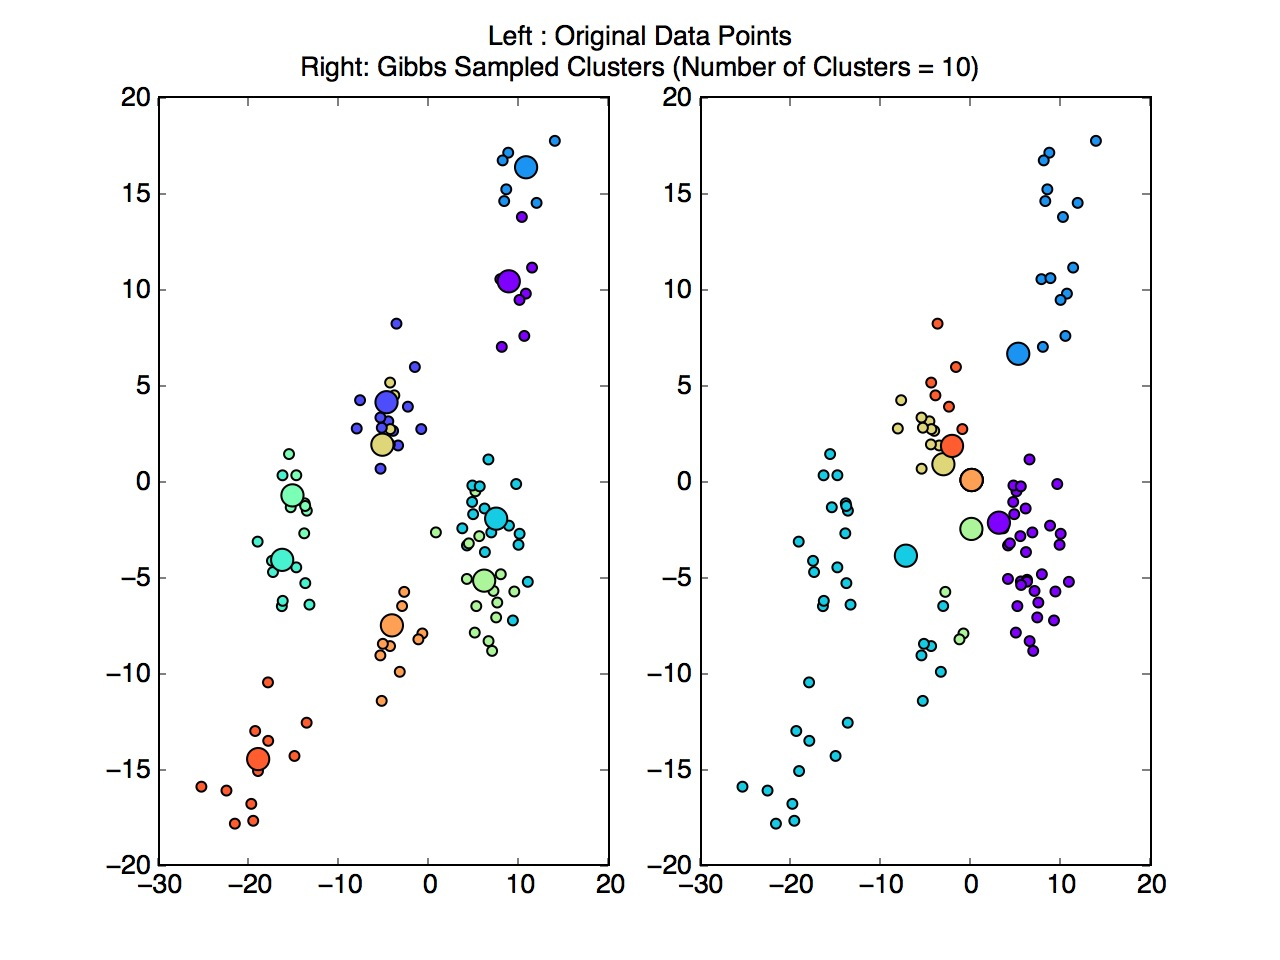
\includegraphics[width=\linewidth]{plot}
	\caption{No. of Iterations : 3000, Burnin : 1000, No. of Points = 100, No. of Clusters = 10}
\end{figure}	

\end{document}

